% Top-level block diagram of P17 on the Zybo Z7-10 (standalone -> block_diagram.pdf)
\documentclass[border=2pt]{standalone}
\usepackage[T1]{fontenc}
\usepackage{lmodern}
\usepackage{tikz}
\usetikzlibrary{arrows.meta,fit,backgrounds,calc}
\begin{document}
\sffamily\footnotesize
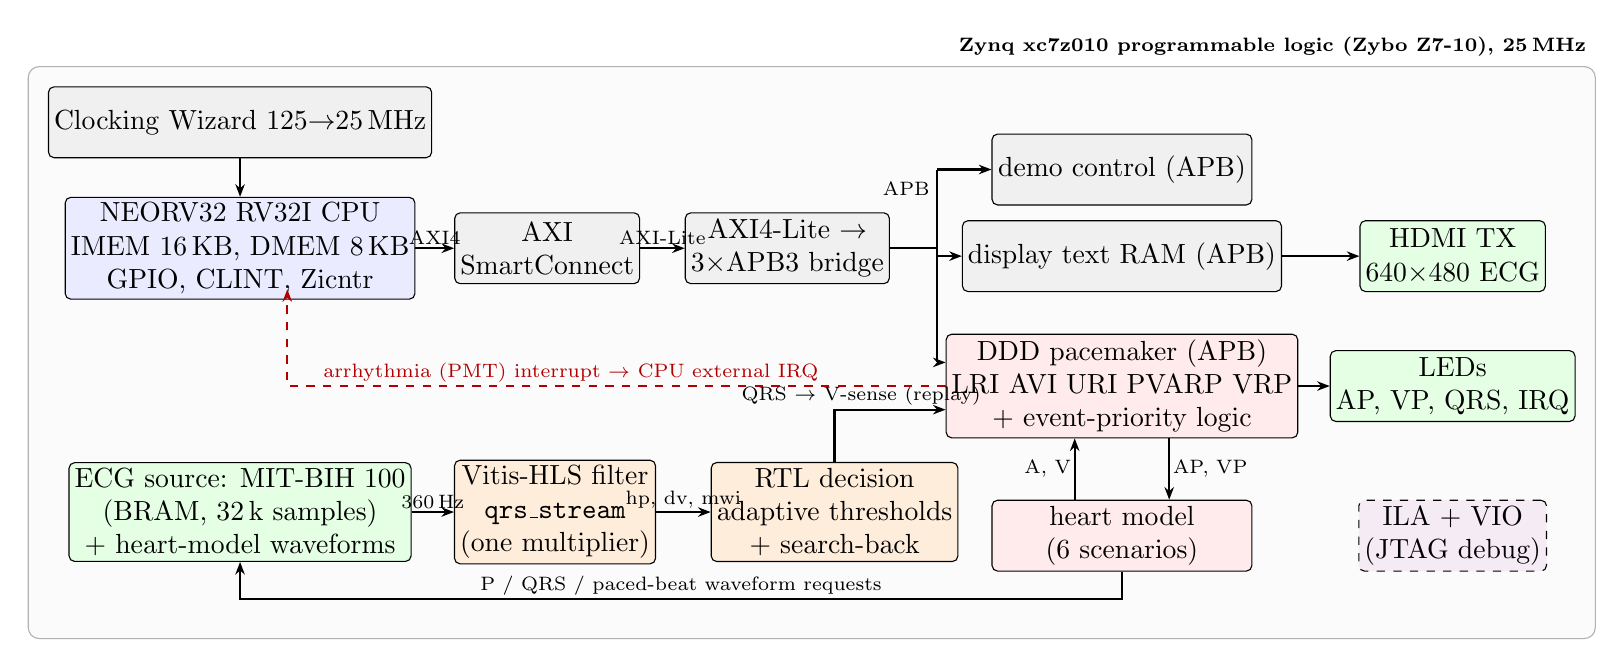
\begin{tikzpicture}[
  blk/.style={draw, rounded corners=2pt, align=center, minimum height=9mm, inner sep=2pt, fill=white},
  cpu/.style={blk, fill=blue!8},
  bus/.style={blk, fill=gray!12},
  acc/.style={blk, fill=orange!14},
  pm/.style={blk, fill=red!8},
  io/.style={blk, fill=green!10},
  dbg/.style={blk, fill=violet!8, dashed},
  ar/.style={-{Stealth[length=1.6mm]}, thick},
  lab/.style={font=\scriptsize, inner sep=1pt}]

% ---------------- row 1: processor, interconnect, APB slaves ----------------
\node[bus, minimum width=31mm] (clk) at (0,1.6) {Clocking Wizard 125$\rightarrow$25\,MHz};
\node[cpu, minimum width=31mm] (cpu) at (0,0) {NEORV32 RV32I CPU\\ IMEM 16\,KB, DMEM 8\,KB\\ GPIO, CLINT, Zicntr};
\node[bus] (sc)  at (3.9,0) {AXI\\SmartConnect};
\node[bus] (br)  at (6.95,0) {AXI4-Lite $\rightarrow$\\ 3$\times$APB3 bridge};
\node[bus, minimum width=33mm] (ctl) at (11.2,1.0)  {demo control (APB)};
\node[bus, minimum width=33mm] (txt) at (11.2,-0.1) {display text RAM (APB)};
\node[pm,  minimum width=33mm] (ddd) at (11.2,-1.75) {DDD pacemaker (APB)\\ LRI AVI URI PVARP VRP\\ + event-priority logic};
\draw[ar] (clk) -- (cpu);
\draw[ar] (cpu) -- node[lab, above]{AXI4} (sc);
\draw[ar] (sc) -- node[lab, above]{AXI-Lite} (br);
\draw[thick] (br.east) -- (8.85,0);
\draw[thick] (8.85,1.0) -- (8.85,-1.45);
\draw[ar] (8.85,1.0) -- (ctl.west);
\draw[ar] (8.85,-0.1) -- (txt.west);
\draw[ar] (8.85,-1.45) -- (ddd.west |- 0,-1.45);
\node[lab, anchor=east] at (8.8,0.75) {APB};

% ---------------- row 2: signal path ----------------
\node[io,  minimum width=31mm] (ecg)   at (0,-3.35) {ECG source: MIT-BIH 100\\ (BRAM, 32\,k samples)\\ + heart-model waveforms};
\node[acc] (hls)   at (4.0,-3.35) {Vitis-HLS filter\\ \texttt{qrs\_stream}\\ (one multiplier)};
\node[acc] (dec)   at (7.55,-3.35) {RTL decision\\ adaptive thresholds\\ + search-back};
\node[pm,  minimum width=33mm] (heart) at (11.2,-3.65) {heart model\\ (6 scenarios)};
\draw[ar] (ecg) -- node[lab, above]{360\,Hz} (hls);
\draw[ar] (hls) -- node[lab, above]{hp, dv, mwi} (dec);
\draw[ar] (dec.north) |- node[lab, pos=0.62, above]{QRS $\rightarrow$ V-sense (replay)} (ddd.west |- 0,-2.05);
\draw[ar] ([xshift=6mm]ddd.south) -- node[lab, right]{AP, VP} ([xshift=6mm]heart.north);
\draw[ar] ([xshift=-6mm]heart.north) -- node[lab, left]{A, V} ([xshift=-6mm]ddd.south);
\draw[ar] (heart.south) -- ++(0,-0.35) -| node[lab, pos=0.25, above]{P / QRS / paced-beat waveform requests} (ecg.south);

% ---------------- interrupt ----------------
\draw[ar, red!70!black, dashed] (ddd.west |- 0,-1.75) -- (0.6,-1.75) -- (0.6,-0.52);
\node[lab, red!70!black, anchor=south] at (4.2,-1.75) {arrhythmia (PMT) interrupt $\rightarrow$ CPU external IRQ};

% ---------------- outputs ----------------
\node[io,  minimum width=22mm] (led)  at (15.4,-1.75) {LEDs\\ AP, VP, QRS, IRQ};
\node[io,  minimum width=22mm] (hdmi) at (15.4,-0.1) {HDMI TX\\ 640$\times$480 ECG};
\node[dbg, minimum width=22mm] (ila)  at (15.4,-3.65) {ILA + VIO\\ (JTAG debug)};
\draw[ar] (ddd) -- (led);
\draw[ar] (txt) -- (hdmi);

\coordinate (botpad) at ($(heart.south)+(0,-0.6)$);
\begin{scope}[on background layer]
\node[draw=gray!60, rounded corners=4pt, fill=gray!3, inner sep=2.5mm,
      fit={(clk)(cpu)(ecg)(heart)(ctl)(led)(ila)(botpad)},
      label={[font=\scriptsize\bfseries, anchor=south east]north east:Zynq xc7z010 programmable logic (Zybo Z7-10), 25\,MHz}] {};
\end{scope}
\end{tikzpicture}
\end{document}
